\section{Task 1: The board, the soak test and the camera stand}
\sectionmark{Task 1: Board, soak test and stand}
\label{sec:t1}

\subsection{Purpose, conditions and criterion}

\begin{plain}{Task 1 at a glance}
\textbf{Purpose.} To turn the EE\,105 board into a dependable camera for the laptop. The capture
program (the ``sketch'') is installed on the board, the transfer of pictures is shown to be
reliable, and a stand holds the camera above the desk so that a page can be photographed from
two measured distances: a greater one for the symbol sheets of Task~2 and a smaller one for the
printed lines of Task~4.

\textbf{Before you begin.} Section~\ref{sec:before} is complete on the laptop that will be used
for photography. You have the board in its box, a micro-USB \emph{data} cable, a plastic or
wooden ruler with a centimetre scale, one or two desk lamps, about a dozen books of which one is a
large hardcover, two small towels or cloths, adhesive tape, and access to a printer.

\textbf{Complete when.} (1)~The laptop receives 100 of 100 pictures in the soak test.
(2)~Text in a photograph reads normally, neither mirrored nor upside down. (3)~With a page on
the desk, a whole block of the symbol sheets is in view and the cropping program accepts it.
(4)~With a page on the platform, the widest test line is between 280 and 300 pixels wide, lies
wholly inside the picture, and is sharp. (5)~The record of Section~\ref{sec:t1record} is filled
in.

\textbf{Time.} About three hours, of which the first upload and the calibration take the most.
\end{plain}

\subsection{Open the project and print the material}

\step{Open the project in PowerShell}\label{st:t1open}
% The opening sequence, written out in full. Input wherever a task may begin in a new window.
If a PowerShell window whose prompt begins with \texttt{(.venv)} is still open, use it and go
on to the next step. Otherwise open a new window (click \ui{Start}, type \code|powershell|,
click \ui{Windows PowerShell}) and give the two commands of the opening sequence in it.
\begin{ps}[Opening sequence, command 1 of 2]
cd C:\ee105\camera-to-latex
\end{ps}
\begin{ps}[Opening sequence, command 2 of 2]
.\.venv\Scripts\Activate.ps1
\end{ps}
\checkpoint{The prompt reads:}
\venvprompt


\step{Print the symbol sheets and the test lines}\label{st:print}
Two documents of the repository are printed once and are used by Tasks~1, 2 and~4:
\file{sheets.pdf} (9 pages, each with two blocks of symbols) and \file{test\_lines.pdf} (16
pages, each with five lines). Open the first folder with
\begin{ps}
explorer C:\ee105\camera-to-latex\sheets
\end{ps}
and double-click \file{sheets.pdf}; it opens in the web browser or in a PDF reader. Press
\key{Ctrl}+\key{P}. In the print dialog set the scale to \ui{Actual size} or \ui{100\,\%}
(never \ui{Fit to page} or \ui{Shrink to fit}), choose single-sided printing, and print on plain
white matte paper. Then open the second folder,
\begin{ps}
explorer C:\ee105\camera-to-latex\test_set
\end{ps}
and print \file{test\_lines.pdf} in the same way. Print pages 1, 6 and 11 of the test lines a
second time; the second copies are the cards of the demonstration (Tasks~5 and~6).
\checkpoint{Measure two lengths with the ruler. On page~8 of the test lines, the line
$y=ax^{2}+bx+c$ (marked T39 at the right margin) is 9.7\,cm long from the leftmost to the
rightmost ink, to within 1\,mm. On page~1 of the sheets, the upper block is 12.7\,cm wide
between the outer edges of its two upper corner squares. If either length is smaller, the
printer has scaled the page: print again at 100\,\%.}

\rationale{All distances in this task are derived from the printed sizes. A page that was
shrunk by a few per cent would still work, but the measurements below would no longer agree
with their predictions, and a fault of the stand could then not be told from a fault of the
print.}

\subsection{Install the Arduino software}

The \term{Arduino IDE} is the program that translates a sketch and transfers it to the board.
It is needed only on the laptop that uploads the sketch, and only for this section: a board
that has been programmed keeps its sketch when it is unplugged.

\step{Install the Arduino IDE}
In a PowerShell window run:
\begin{ps}
winget install --id ArduinoSA.IDE.stable -e --source winget
\end{ps}
Answer \ui{Yes} if the \ui{User Account Control} dialog appears. When the installation has
finished, click \ui{Start}, type \code|arduino| and click \ui{Arduino IDE}. During its first
start, Windows may ask whether the program may use the network (either answer is acceptable,
because the board is reached through the cable) and, several times, whether to install device
software from Arduino; click \ui{Install} each time.
\checkpoint{The Arduino IDE window is open and shows an empty sketch that contains the words
\texttt{void setup()} and \texttt{void loop()}.}

\begin{iffail}
If winget cannot find the package, download the installer from
\url{https://www.arduino.cc/en/software} (the entry for Windows~10 and newer, 64 bits), run it
with the settings it proposes, and continue with the next step.
\end{iffail}

\step{Install the board package}
The IDE must be told about the board's processor. In the narrow column of icons at the left
edge of the window, click the second icon from the top; when the mouse rests on it, the tooltip
\ui{Boards Manager} appears. Type \code|mbed nano| in the search box. In the entry \ui{Arduino
Mbed OS Nano Boards}, by Arduino, click \ui{INSTALL}. The download is large and takes several
minutes; the panel at the bottom of the window reports the progress. Answer \ui{Yes} or
\ui{Install} to any question from Windows. (If the IDE itself offers at some later moment to
install this package for the connected board, accept the offer; the result is the same.)
\checkpoint{The entry shows a \ui{REMOVE} button in place of the \ui{INSTALL} button.}

\step{Install the camera library}
Click the third icon of the left column (tooltip \ui{Library Manager}). Type
\code|Arduino_OV767X| in the search box. In the entry \ui{Arduino\_OV767X}, by Arduino, click
\ui{INSTALL}.
\checkpoint{The entry shows \ui{REMOVE}, and its version is 0.0.2 or later.}

\subsection{Connect the board}

\begin{figure}[H]
\centering
\begin{tikzpicture}
\node[anchor=south west, inner sep=0] (img) at (0,0) {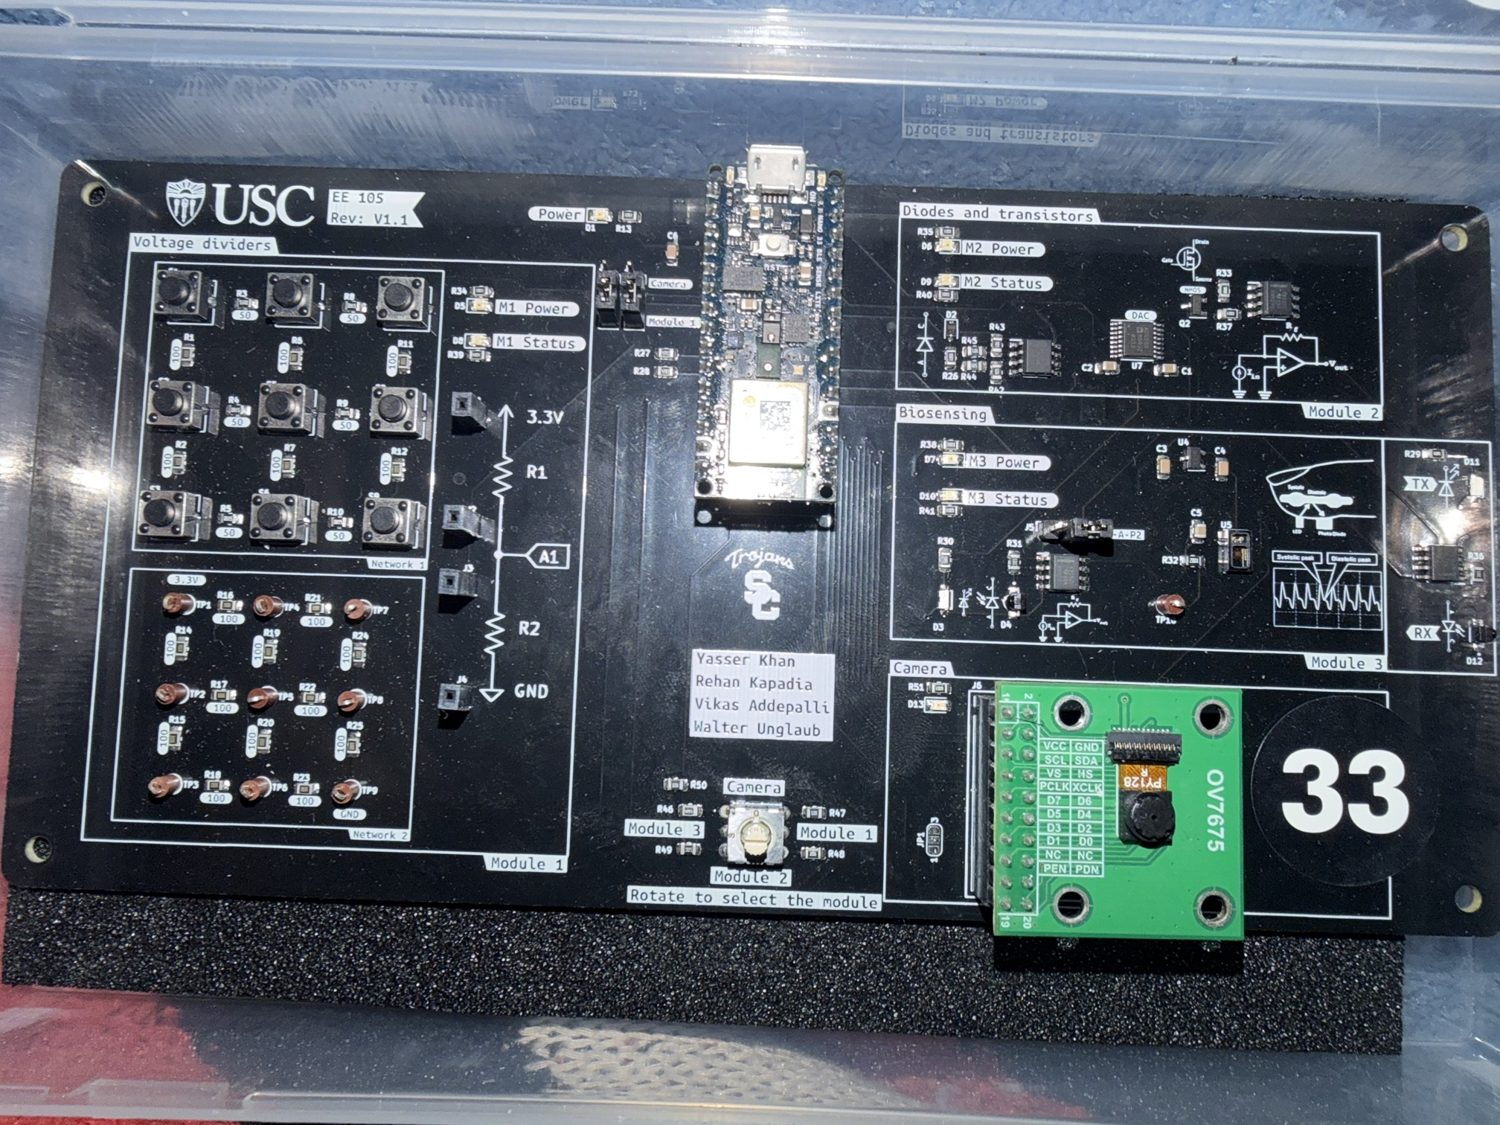
\includegraphics[width=\linewidth]{img/board.jpg}};
\begin{scope}[x={(img.south east)}, y={(img.north west)},
  lab/.style={fill=white, draw=black!70, rounded corners=1.5pt, inner sep=2.5pt, font=\sffamily\scriptsize, align=center},
  ptr/.style={-{Stealth[length=2mm]}, line width=0.9pt, white, double=black, double distance=0.5pt}]
\node[lab] (cam) at (0.86,0.07) {A\ \ camera lens};
\draw[ptr] (cam) -- (0.775,0.245);
\node[lab] (nano) at (0.78,0.955) {B\ \ Arduino Nano, with the USB socket};
\draw[ptr] (nano.west) -- (0.535,0.865);
\node[lab] (sel) at (0.42,0.07) {C\ \ module selector};
\draw[ptr] (sel) -- (0.495,0.235);
\node[lab] (jmp) at (0.22,0.955) {D\ \ two jumpers};
\draw[ptr] (jmp.south) -- (0.405,0.755);
\node[lab] (but) at (0.12,0.07) {E\ \ supported end};
\draw[ptr] (but) -- (0.10,0.30);
\end{scope}
\end{tikzpicture}
\caption{The EE\,105 board, seen from its component side. The camera~(A) looks out of the page.
The laptop is connected at the micro-USB socket of the Arduino Nano~(B). The selector~(C) must
point to \emph{Camera}. The jumpers~(D) stay as they were in the digit-recognition laboratory.
In the stand of Section~\ref{sec:stand} the board lies face down and rests on its end~(E).}
\label{fig:board}
\end{figure}

\step{Set the selector and connect the cable}
Take the board out of its box by its edges and lay it, components upwards, on a dry table of
wood or plastic. Find the rotary selector~(C in Figure~\ref{fig:board}), which is labelled
\emph{Rotate to select the module}, and turn it until its mark points to \ui{Camera}. Leave
the two small black jumpers beside the Nano~(D) where they are: they were set for the camera
during the digit-recognition laboratory. If a transparent protective film covers the camera
lens~(A), peel it off. Plug the small end of the USB cable into the socket of the Nano~(B) and
the other end into the laptop, directly and not through a hub or a docking station.
\checkpoint{A small light is lit on the board, and Windows has played its ``device connected''
sound.}

\begin{iffail}
If nothing lights up, try another USB socket of the laptop and then another cable. Many
micro-USB cables are made for charging only and carry no data; with such a cable the light
comes on, but the board never appears in the list of ports in Step~\ref{st:port}.
\end{iffail}

\subsection{Upload the sketch}

\step{Open the sketch}
In the Arduino IDE choose \menu{File}\then\menu{Open\ldots}, go to the folder
\file{C:\bs ee105\bs camera-to-latex\bs firmware\bs capture}, select \file{capture.ino} and
click \ui{Open}. The sketch appears in a new window; the empty window may be closed.

\step{Check that the sketch names the right camera}\label{st:model}
Near the top of the sketch, below the line that contains the word \emph{settings}, look for a
line that begins as follows.
\begin{filebox}{Sketch capture.ino: the first setting}
#define CAMERA_MODEL  OV7675
\end{filebox}
\checkpoint{The line is present.}
\rationale{The camera library supports two sensors and assumes the older OV7670 unless it is
told otherwise. Copies of the sketch made before 24 November 2026 lack this line and therefore
configure the board's OV7675 with the settings of the wrong sensor.}
\begin{iffail}[If the line is missing]
Your copy of the repository is out of date. Close the sketch window, carry out
Step~\ref{st:uptodate}, and open the sketch again.
\end{iffail}

\step{Select the board and the port}\label{st:port}
Choose \menu{Tools}\then\menu{Board}\then\menu{Arduino Mbed OS Nano Boards}\then\menu{Arduino
Nano 33 BLE}. (The Sense Lite has no entry of its own; it is programmed as a Nano 33 BLE.) Then
choose \menu{Tools}\then\menu{Port} and click the entry that names the board, for example
\emph{COM5 (Arduino Nano 33 BLE)}. Write the port name down.
\checkpoint{The bottom right corner of the IDE window shows \emph{Arduino Nano 33 BLE on COM}
followed by a number.}

\step{Upload}\label{st:upload}
Click the round button with the arrow that points to the right, at the top left of the window
(tooltip \ui{Upload}). The IDE first translates the sketch, which takes between two and ten
minutes the first time, and then transfers it, which takes a few seconds. During the transfer
the port may disappear and reappear, sometimes under a different number. A warning that little
memory is left may appear; it is harmless, because the sketch deliberately reserves most of the
board's memory for one picture.
\checkpoint{The IDE shows the message \emph{Done uploading}.}

\begin{iffail}[If the upload fails or never starts]
Press the small white button on the Nano twice in quick succession. An orange light on the Nano
then fades in and out, which shows that the board is waiting for a program. Select the port
again (\menu{Tools}\then\menu{Port}; its number may have changed) and click \ui{Upload} once
more.
\end{iffail}

\step{Release the port}
Close the Arduino IDE completely.
\rationale{Only one program at a time can use a serial port. As long as the IDE, or its
\emph{Serial Monitor}, holds the port, the Python programs of the following steps are refused
with the message \emph{Access is denied}.}

\subsection{Test the link between board and laptop}

The remaining steps of this task are given in the PowerShell window of Step~\ref{st:t1open}. If
that window has been closed in the meantime, carry out Step~\ref{st:t1open} again first.

\step{List the serial ports}
\begin{ps}
python -m pipeline.capture --list
\end{ps}
\begin{out}[What you should see (the port number will differ)]
COM5                     USB Serial Device (COM5)  vid=9025 pid=32858
\end{out}
\checkpoint{One line shows \texttt{vid=9025}, the identification number of Arduino. Other
lines, for example for Bluetooth devices, may appear as well.}

\step{Ask the board whether it is alive}\label{st:ping}
\begin{ps}
python -m pipeline.capture --ping
\end{ps}
\begin{out}
port COM5
board answers: 320x240, 1 byte(s) per pixel
\end{out}
\checkpoint{The second line appears within a few seconds.}

\begin{iffail}
If this is the first command since the board was plugged in, give it a second time before
drawing any conclusion: the camera needs a moment to start when the port is opened for the
first time. Otherwise the answer names the cause. \emph{Access is denied}: another program
holds the port; close the Arduino IDE. \emph{cannot pick the board's port automatically}: more than one candidate is
connected; unplug other Arduino boards, or name the port by adding it to the command, as in
\code|python -m pipeline.capture --ping --port COM5|. \emph{unexpected ping answer: ERR
camera}: the sketch runs but cannot start the camera; see Section~\ref{sec:t1trouble}.
\emph{no answer}: the sketch is not on the board; repeat Step~\ref{st:upload}.
\end{iffail}

\subsection{First pictures and orientation}

\step{Open the viewfinder}\label{st:viewfinder}
\begin{ps}
python -m pipeline.capture --series data\raw\rig --names "first"
\end{ps}
A window with the title \emph{capture series} opens and shows what the camera sees, enlarged
twofold. The yellow line at the top names the photograph that will be saved next, and the line
at the bottom lists the keys (Table~\ref{tab:serieskeys}). Three properties of this window
matter throughout Tasks~1, 2 and~4.
\begin{itemize}
\item The picture is renewed only about once per second. After moving anything, wait until the
  picture has changed and then stood still for two seconds before judging or saving it.
\item The keys act only while this window is the active one: click once on the picture first.
\item The keys are lower-case letters. If they have no effect, the \key{Caps Lock} key is on.
\end{itemize}

\begin{table}[H]
\centering
\begin{tabular}{C{2.2cm}L{8.6cm}}
\toprule
\hd{Key} & \multicolumn{1}{c}{\hd{Effect in the capture-series window}} \\
\midrule
\key{Space} & Save the current picture under the name shown, and go on to the next name \\
\key{B} & Go back one name, so that a photograph can be taken again \\
\key{N} & Skip the current name without saving \\
\key{Q} or \key{Esc} & Close the window \\
\bottomrule
\end{tabular}
\caption{Keys of the capture-series window. After the last name of its list, the window closes
by itself.}
\label{tab:serieskeys}
\end{table}

Hold the board by its edges about 15\,cm above a printed page of test lines, with the camera
looking down at the page and a lamp lighting the page, and move it until a line is in view.
\checkpoint{Printed characters can be recognized in the window, even if they are upside down,
mirrored or slightly blurred. A picture of noise or stripes, or a uniformly gray picture, is a
failure: see Section~\ref{sec:t1trouble}.}

\step{Test for a mirror image}\label{st:orient}
Turn the \emph{page} until the text in the window stands upright, and look at the letters.
\begin{itemize}
\item If they read normally, no setting is needed.
\item If they are reversed as in a mirror, the setting \code|FLIP_H| must become \code|True|.
  Press \key{Q} to close the window, change the setting as described in
  Section~\ref{sec:setting}, and repeat Step~\ref{st:viewfinder} to confirm that the text now
  reads normally.
\end{itemize}
Finally press \key{Space} to save one photograph, which also closes the window.
\checkpoint{Upright text in the viewfinder reads normally, PowerShell has printed \emph{saved
first.png}, and the file exists in the folder \file{data\bs raw\bs rig}.}

\rationale{A sensor may deliver its lines in either direction, so a mirror image cannot be
excluded in advance; it can be undone only by this setting. An image that is merely upside
down needs no setting, because the page can be turned. Photographs are stored exactly as the
camera delivers them, and the setting is applied whenever a photograph is read; a correction
made later therefore also holds for photographs taken earlier.}

\subsection{The soak test}

\step{Request one hundred pictures}\label{st:soak}
Lay the board, components upwards, on the wooden or plastic table, with a lit page or wall in
front of the camera, and run:
\begin{ps}
python -m pipeline.capture --soak 100
\end{ps}
The command requests 100 pictures in succession and verifies each one by its \term{checksum},
the sum of all its pixel values, which the board transmits after the pixels. It runs for two to
four minutes.
\begin{out}[What you should see (the measured values will differ)]
port COM5
first frame 320x240, mean level 121
100/100 frames OK, 0 failed, 1.31 s per frame
\end{out}
\checkpoint{The last line begins with \texttt{100/100 frames OK}. Enter the time per frame in
the record.}

\begin{iffail}[If some pictures fail]
Each failure is reported on a line of its own with its reason (\emph{timeout} or \emph{checksum
mismatch}). Connect the board to a socket of the laptop itself, use a shorter cable, and repeat
the test. The application repeats a failed request up to three times, so that one or two
failures in a hundred do not prevent further work; the criterion of this task, however, is a
clean run. If failures persist, enter their number in the record and inform the lead.
\end{iffail}

\subsection{Build the stand}
\label{sec:stand}

\subsubsection*{Requirements}

Any construction is acceptable that meets the following five requirements.
\begin{enumerate}
\item The lens looks straight down at the desk from a height of 16 to 18\,cm, and stays there
  when the cable or the page is touched.
\item Around the point of the desk directly below the lens, at least 20\,cm are free in every
  direction, so that a printed page can be moved to bring any of its lines below the lens.
\item The page can lie at two distances from the lens: on the desk, and on a firm platform 5 to
  7\,cm thick.
\item Nothing conductive touches the board, and nothing presses on the camera or on the Nano.
\item The USB cable is fastened to the stand, so that a pull on the cable cannot move the
  board.
\end{enumerate}
The camera is fixed and the \emph{page} is raised for close work, because a platform of books is
easier to rebuild exactly than a stand of adjustable height.

\subsubsection*{A construction from books}

Figure~\ref{fig:stand} shows a stand that needs only books, two cloths and tape. A large
hardcover book projects from a stack like an arm, and the board lies face down on the end of
the arm.

\begin{figure}[H]
\centering
\begin{tikzpicture}[x=0.22cm, y=0.22cm, font=\scriptsize, >={Stealth[length=1.6mm]}]
% desk
\draw[line width=0.9pt] (-1,0) -- (52.5,0);
% base stack
\fill[black!14] (0,0) rectangle (18,14); \draw (0,0) rectangle (18,14);
\foreach \y in {2.8,5.6,8.4,11.2} \draw[black!45] (0,\y) -- (18,\y);
% arm
\fill[black!32] (3,14) rectangle (31,17); \draw (3,14) rectangle (31,17);
% weights on the arm
\fill[black!14] (3,17) rectangle (16.5,23); \draw (3,17) rectangle (16.5,23);
\foreach \y in {19,21} \draw[black!45] (3,\y) -- (16.5,\y);
% cloth, board, cloth, light weight
\fill[black!60] (25.6,17) rectangle (31,17.45);
\fill[green!40!black] (26,17.45) rectangle (43.5,17.8);
\fill[black!60] (25.6,17.8) rectangle (31,18.25);
\fill[black!14] (25.9,18.25) rectangle (30.7,20.6); \draw (25.9,18.25) rectangle (30.7,20.6);
% camera
\fill[black] (38.6,16.75) rectangle (40.4,17.45);
\fill[black] (39.2,16.3) rectangle (39.8,16.75);
% platform and pages
\fill[black!7] (30.5,0) rectangle (48.5,5.6); \draw[densely dashed] (30.5,0) rectangle (48.5,5.6);
\draw[line width=1.3pt] (31.5,5.75) -- (47.5,5.75);
\draw[line width=1.3pt, black!55] (29.5,0.15) -- (49.5,0.15);
% view
\draw[densely dotted, line width=0.6pt] (39.5,16.3) -- (31.6,0.15);
\draw[densely dotted, line width=0.6pt] (39.5,16.3) -- (47.4,0.15);
% dimensions
\draw[<->] (50.6,0) -- (50.6,16.3);
\draw[black!55] (39.9,16.3) -- (50.9,16.3);
\node[anchor=west, align=left] at (50.7,10.4) {16 to\\18\,cm};
\draw[<->] (44.9,5.75) -- (44.9,16.3);
\node[anchor=west, align=left] at (45.0,12.6) {about\\11\,cm};
\draw[<->] (18,9.3) -- (39.5,9.3);
\draw[black!55, densely dashed] (39.5,16.2) -- (39.5,6.2);
\node[anchor=south] at (27.6,9.3) {20\,cm or more};
% labels
\node[align=center] at (9,7) {base stack};
\node[align=center] at (9.7,20.1) {heavy books};
\node[anchor=west] at (4,15.5) {arm: a large hardcover book};
\node[anchor=south, align=center] (bl) at (36.8,20.6) {board, face down,\\between two cloths};
\draw[->] (bl.south) -- (35.3,18.0);
\node[anchor=south, align=center] (wl) at (25.5,23.4) {light book};
\draw[->] (wl.south) -- (28.2,20.8);
\node[anchor=north, align=center] (cl) at (35.2,14.9) {lens};
\draw[->] (cl.east) -- (39.0,16.4);
\node[anchor=north, align=center] at (39.5,-0.4) {platform (for lines only), page on top};
\node[anchor=north, align=center] at (9,-0.4) {desk};
\end{tikzpicture}
\caption{Side view of a stand built from books. For the symbol sheets the page lies on the desk,
16 to 18\,cm below the lens (\emph{sheet position}). For the test lines the page lies on a
platform that brings it to about 11\,cm below the lens (\emph{line position}). The dotted lines
show the camera's view.}
\label{fig:stand}
\end{figure}

\step{Build the stack and the arm}
On a desk, stack books to a height of about 14\,cm, with one straight vertical face. Lay a large
hardcover book, the \emph{arm}, on top, so that it projects 12 to 15\,cm beyond that face, and
lay two or three heavy books on the part of the arm that rests on the stack.
\checkpoint{The projecting end of the arm does not sink or rock when it is pressed down gently
with a finger, and its upper surface is 17 to 18\,cm above the desk.}

\step{Place the board}
Unplug the USB cable from the laptop. Lay a folded dry cloth on the projecting end of the arm.
Turn the board over and lay it on the cloth with its components downwards and its long side in
line with the arm, so that the end marked~E in Figure~\ref{fig:board} rests on the arm over a
length of 4 to 5\,cm and the rest of the board, with the Nano and the camera, projects freely
beyond the arm. Lay the second folded cloth on the supported end and a paperback book on it.
\checkpoint{Seen from the side, the board is level, and nothing touches the camera or the Nano.
Stand the ruler on the desk beside the camera: the front of the lens is between 16 and 18\,cm
above the desk. Add or remove a thin book of the base stack to correct the height.}

\step{Fasten the cable}
Plug the cable into the laptop again. Lead it from the Nano back along the arm, leaving a loose
bend of a few centimetres at the plug, and tape it to the arm.
\checkpoint{A gentle pull on the cable beyond the tape does not move the board.}

\step{Place a white background and the lamp}
Lay two blank white sheets on the desk below the camera, so that the camera sees only white
paper wherever no printed page lies. Place the lamp, or better two lamps, to the left and to
the right of the board at a distance of 30 to 40\,cm, with their heads no higher than the
board, so that the light falls on the paper at a shallow angle from the side.
\begin{ps}
python -m pipeline.capture --series data\raw\rig --names "blank"
\end{ps}
Look at the viewfinder. The picture should be an even light gray. A darker region with a sharp
border is the shadow of the board, of the cable or of the arm: move the lamp until it has left
the picture. A white spot is the reflection of the lamp: lower the lamp or move it farther to
the side. Then press \key{Space}.
\checkpoint{The viewfinder shows an evenly lit, empty sheet, without shadows and without bright
spots, and \emph{saved blank.png} has been printed.}

\step{Find the direction of the page}\label{st:pagedir}
\begin{ps}
python -m pipeline.capture --series data\raw\rig --names "direction"
\end{ps}
Lay page~1 of the printed test lines below the camera and turn it in steps of a quarter turn
until its text stands upright in the viewfinder and runs from left to right. Stick a strip of
tape on the desk and draw on it an arrow that points towards the top edge of the page as it now
lies. Press \key{Space}.
\checkpoint{The arrow on the desk shows where the top of every page must point from now on.}

\subsection{Calibrate the two positions}

\subsubsection*{Geometry}

The calibration measures the \term{scale} $s$ of a photograph, the number of pixels that one
centimetre of paper occupies. The scale follows from the distance $d$ between the lens and the
page. A lens with a horizontal angle of view $\theta$ sees a strip of paper of width
\[
  w = 2\,d\,\tan\frac{\theta}{2} = k\,d ,
\]
and this strip is spread over the 320 pixels of the long side of the picture, so that
\[
  s = \frac{320}{w} = \frac{320}{k\,d} .
\]
A printed length $\ell$ then appears with $\ell\,s$ pixels. For the lens of this board the
published angles of view give a constant $k$ between 0.89 and 1.0. Two printed lengths matter:
the height of a capital letter, 0.96\,cm at the print size of 40\,pt, and the width of the
widest test line, T39, which is 9.67\,cm. Table~\ref{tab:geometry} lists what the formula
predicts for them; the calibration replaces these predictions by measurements.

\begin{table}[H]
\centering
\begin{tabular}{C{1.7cm}C{2.5cm}C{2.2cm}C{2.0cm}C{2.0cm}}
\toprule
\hd{Distance $d$} & \hd{Width in view $w$} & \hd{Scale $s$} & \hd{Capital height} & \hd{Width of T39} \\
\midrule
17 cm & 15.1--17.0 cm & 19--21 px/cm & 18--20 px & 182--205 px \\
15 cm & 13.4--15.0 cm & 21--24 px/cm & 20--23 px & 206--232 px \\
13 cm & 11.6--13.0 cm & 25--28 px/cm & 24--27 px & 238--267 px \\
12 cm & 10.7--12.0 cm & 27--30 px/cm & 26--29 px & 258--290 px \\
11 cm & 9.8--11.0 cm & 29--33 px/cm & 28--31 px & 281--316 px \\
10 cm & 8.9--10.0 cm & 32--36 px/cm & 31--35 px & 309--348 px \\
\bottomrule
\end{tabular}
\caption{Predicted size of printed material in the photograph, for material printed at 40\,pt.
The depth of the view is three quarters of its width.}
\label{tab:geometry}
\end{table}

Two requirements fix the two positions. A block of the symbol sheets measures $12.7 \times
10.0$\,cm including its corner squares; to show it whole, the view must be at least
$13.5 \times 10.8$\,cm, which the table places at a distance of 16 to 18\,cm. This is the
\emph{sheet position}. For the test lines, larger letters are read more reliably. In simulated
photographs read with the fallback classifier, 57 of the 80 lines were read exactly when
capitals were 24 pixels tall, 63 at 28 pixels and 65 at 30 pixels; of the nine lines of plain
text, one, four and six. The picture, however, is only 320 pixels wide, and line T39 is 10.1
capital heights long: it occupies 282 pixels when capitals are 28 pixels tall and 302 pixels
when they are 30. The \emph{line position} is therefore the distance at which line T39 is
between 280 and 300 pixels wide, which corresponds to a scale of 29 to 31\,px/cm and to
capitals of 28 to 30 pixels; the table places it at 11 to 12\,cm. (The update report named a
provisional height of about 12.5\,cm and capitals of 30 pixels or more. The analysis above
refines both figures: at 12.5\,cm capitals would measure only 25 to 28 pixels, and above 30
pixels line T39 no longer fits into the picture.)

\subsubsection*{The sheet position}

\step{Photograph a ruler and a block on the desk}\label{st:calsheet}
\begin{ps}
python -m pipeline.capture --series data\raw\rig --names "desk_ruler,A1_0"
\end{ps}
For the first photograph, lay the ruler on the white sheet below the camera, parallel to the
long side of the picture, so that its centimetre scale crosses the whole picture; press
\key{Space}. For the second, remove the ruler and lay page~1 of the printed symbol sheets on the
desk, its top towards the arrow, so that its upper block is in the middle of the picture. The
small words below each block give its name; this one is block~A1. Cover the lower block of the
page with a blank sheet whose edge runs through the middle of the white gap between the two
blocks. Check in the viewfinder that all four corner squares are inside the picture, that the
hollow square is at the top left, and that white paper is visible between each square and the
border of the picture; then press \key{Space}.
\checkpoint{PowerShell has printed \emph{saved desk\_ruler.png} and \emph{saved A1\_0.png}.}

\begin{iffail}[If the four corner squares do not fit into the picture]
The camera is too low. Add a thin book to the base stack and repeat this step. If, on the
contrary, the block occupies less than three quarters of the width of the picture, the camera is
higher than necessary: remove a book.
\end{iffail}

\step{Measure the scale on the desk}\label{st:paint}
\begin{ps}
mspaint data\raw\rig\desk_ruler.png
\end{ps}
The photograph opens in Paint. Enlarge it with the slider at the bottom right of the window
until the centimetre marks can be told apart. Rest the tip of the pointer on the mark of 2\,cm
and read the two numbers at the bottom left of the window: they are the position of the
pointer in pixels, counted from the left and from the top of the photograph. Note the first
number, $x_1$. Do the same on the mark of 12\,cm for $x_2$. The scale on the desk is
\[
  s_{\text{desk}} = \frac{x_2 - x_1}{10\ \text{cm}} .
\]
For example, positions of 41 and 243 give a scale of 20.2\,px/cm and a view that is
$320/20.2 = 15.8$\,cm wide. Close Paint without saving. (Paint shows the photograph as it is
stored. If the setting \code|FLIP_H| is \code|True|, the stored photograph is the mirror image
of what the viewfinder showed; distances between marks are not affected.)
\checkpoint{The scale is between 18 and 23\,px/cm. Enter it in the record.}

\begin{iffail}[If Paint does not open the photograph]
Open the folder with the command \code|explorer data\raw\rig|, right-click the file
\file{desk\_ruler.png} and choose \menu{Open with}\then\menu{Paint}.
\end{iffail}

\step{Let the cropping program judge the block}\label{st:calcrop}
\begin{ps}
python -m tools.crop_sheet --photos data\raw\rig --out data\raw\rig\crops
\end{ps}
\begin{out}[What you should see (the number of pixels will differ)]
A1_0.png: 35 crops, capitals 20 px

35 crops from 1 photos -> data\raw\rig\crops
\end{out}
\checkpoint{The line for \file{A1\_0.png} reports 35 crops; the words \emph{read as an upright
page} may follow and are acceptable. The stand is now at a usable sheet position. Measure the
height of the lens above the desk once more and enter it in the record.}

\begin{iffail}
The word \emph{skipped}, followed by a reason in parentheses, means that the program did not
find the four corner squares. Repeat Step~\ref{st:calsheet} with more white paper around the
block, with the page lying flat, and without a shadow on any corner.
\end{iffail}

\subsubsection*{The line position}

\step{Build the platform and photograph line T39}\label{st:calline}
Lay flat books below the camera to a height of 6\,cm, with a blank white sheet on top. This is
the \emph{platform}. Lay page~8 of the printed test lines on it, its top towards the arrow; the
names of the lines are printed small at the right margin of the page.
\begin{ps}
python -m pipeline.capture --series data\raw\rig --names "p1_T39"
\end{ps}
Move the page until line T39, $y=ax^{2}+bx+c$, lies in the middle of the picture, with equal
white margins to its left and right. Parts of the lines above and below it may show at the
upper and lower borders of the picture; they do no harm and are not to be covered. Press
\key{Space}.
\checkpoint{\emph{saved p1\_T39.png} has been printed.}

\rationale{The program keeps only the row of ink nearest the middle of the picture. In 240
simulated photographs, the number of lines read exactly was the same, 196, whether the
neighbouring lines of the page were present or not; an aim that was 7\,mm too high or too low
changed it by at most two.}

\step{Measure the width of the line}\label{st:measure}
\begin{ps}
mspaint data\raw\rig\p1_T39.png
\end{ps}
Enlarge the picture as far as the slider allows. Rest the pointer on the leftmost dark pixel of
the line and note the first number at the bottom left, $x_{\text{left}}$. Rest it on the
rightmost dark pixel of the line and note $x_{\text{right}}$. Then
\[
  W = x_{\text{right}} - x_{\text{left}} + 1, \qquad
  s_{\text{line}} = \frac{W}{9.67\ \text{cm}}, \qquad
  h \approx \frac{W}{10} ,
\]
where $W$ is the width of the line, $s_{\text{line}}$ the scale and $h$ the height of a capital
letter, all in pixels. The white margins of the line are $x_{\text{left}}$ on the left and
$319 - x_{\text{right}}$ on the right. While the picture is enlarged, judge its sharpness: the
two bars of the equals sign must be separated by a clearly lighter row of pixels, and the small
2 must be recognizable as a 2. Close Paint without saving.
\checkpoint{$W$, the two margins and the verdict on sharpness are entered in the first row of
Table~\ref{tab:trials}.}

\begin{table}[H]
\centering
\begin{tabular}{C{1.3cm}C{2.3cm}C{1.9cm}C{2.3cm}C{2.5cm}}
\toprule
\hd{Trial} & \hd{Platform} & \hd{Width $W$} & \hd{Margins} & \hd{Sharp?} \\
\midrule
p1 & \hfill cm & \hfill px & \hfill px & \cbox\ yes\quad\cbox\ no \\
p2 & \hfill cm & \hfill px & \hfill px & \cbox\ yes\quad\cbox\ no \\
p3 & \hfill cm & \hfill px & \hfill px & \cbox\ yes\quad\cbox\ no \\
p4 & \hfill cm & \hfill px & \hfill px & \cbox\ yes\quad\cbox\ no \\
\bottomrule
\end{tabular}
\caption{Trials of the line position. The platform is described by its thickness.}
\label{tab:trials}
\end{table}

\step{Adjust the platform until the criteria are met}\label{st:adjust}
The criteria are: $W$ from 280 to 300 pixels; both margins at least 10 pixels; a sharp picture.
Because the size of the image is inversely proportional to the distance, a small change
$\Delta d$ of the distance changes the width by
\[
  \Delta W \approx -\,\frac{W}{d}\,\Delta d ,
\]
which near the target amounts to about 10 pixels for every 4\,mm. If $W$ is below 280, raise
the platform by 4\,mm, the thickness of a thin notebook or magazine, for every 10 pixels that
are missing; if it is above 300, lower it likewise. Then photograph and measure again under a
new name, so that the earlier photographs are kept for comparison:
\begin{ps}[Second trial]
python -m pipeline.capture --series data\raw\rig --names "p2_T39"
\end{ps}
\begin{ps}[To measure the second trial]
mspaint data\raw\rig\p2_T39.png
\end{ps}
For a third and a fourth trial, write \code|p3_T39| and \code|p4_T39| in place of
\code|p2_T39| in both commands.
\checkpoint{One trial meets all three criteria. Its platform is the \emph{line platform}: keep
its books together, mark the pile, and outline its position on the desk with tape so that it
can be put back exactly.}

\begin{iffail}[If the picture is blurred at 280 pixels but sharp when the page lies lower]
The lens cannot focus at so short a distance. Find the thickest platform at which the picture
is sharp, and enlarge the print instead of approaching it: carry out
Section~\ref{sec:bigprint} before anything is photographed for Tasks~2 and~4.
\end{iffail}

\subsection{Acceptance test with the application}

\step{Read five probe lines through the complete pipeline}\label{st:accept}
With the line platform in place, start the application:
\begin{ps}
python -m pipeline.main --new
\end{ps}
After up to half a minute, a window with the title \emph{camera to latex} shows the live
picture;
below it, two lines of text give the state of the program and its keys. Bring one of the lines
of Table~\ref{tab:probes} into the middle of the picture, wait until the picture stands still,
and press \key{Space}. The picture freezes. A box is drawn around every symbol that was found:
green where the classifier is confident, red where it is not, blue for the bar of a fraction.
The name that the classifier gives each symbol is written above its box, and the reading of the
whole line appears below the picture and in the PowerShell window. Press \key{R} to return to
the live picture. Do this for the five lines of the table, then press \key{Q}.

\begin{table}[H]
\centering
\begin{tabular}{C{1.4cm}C{3.9cm}C{1.5cm}C{3.6cm}}
\toprule
\hd{Line} & \hd{Printed content} & \hd{Page} & \hd{One box per symbol?} \\
\midrule
D03 & USC Trojans & 13 & \cbox\ yes\quad\cbox\ no \\
D08 & $z=x+iy$ & 14 & \cbox\ yes\quad\cbox\ no \\
D05 & $a^{2}+b^{2}=c^{2}$ & 13 & \cbox\ yes\quad\cbox\ no \\
D14 & $\dfrac{1}{3}+\dfrac{2}{3}=1$ & 15 & \cbox\ yes\quad\cbox\ no \\[6pt]
T39 & $y=ax^{2}+bx+c$ & 8 & \cbox\ yes\quad\cbox\ no \\
\bottomrule
\end{tabular}
\caption{Probe lines for the acceptance test of the stand. The pages are those of the printed
test lines.}
\label{tab:probes}
\end{table}

\checkpoint{For at least four of the five lines, every printed symbol has exactly one box (a
letter with a dot, an equals sign and a fraction bar each count as one symbol), the note
\emph{ink touches the photo edge} does not appear below the picture, and the reading appears
within five seconds of the key press. Whether each symbol is also \emph{named} correctly is not
judged here; that is the subject of Tasks~2 and~3.}

\begin{iffail}
Boxes that split one letter into two, or join two letters into one, on most lines indicate
letters that are too small or too blurred: review the trials of Table~\ref{tab:trials}. The
note about the photo edge means that the line was not wholly inside the picture: centre it and
read it again.
\end{iffail}

\subsection{Record and share}
\label{sec:t1record}

\step{Fill in the record}
\begin{table}[H]
\centering
\begin{tabular}{L{7.0cm}C{4.2cm}}
\toprule
\multicolumn{1}{c}{\hd{Quantity}} & \hd{Value} \\
\midrule
Board number (white disc beside the camera); date & \\
Serial port & \\
Soak test: pictures received of 100; time per picture & \\
Setting \texttt{FLIP\_H} (True or False) & \\
Height of the lens above the desk & \hfill cm \\
Scale on the desk, $s_{\text{desk}}$ & \hfill px/cm \\
Capital height reported by the cropping program & \hfill px \\
Thickness of the line platform & \hfill cm \\
Distance from the lens to the page on the platform & \hfill cm \\
Width $W$ of line T39 on the platform & \hfill px \\
Scale on the platform, $s_{\text{line}} = W / 9.67$\,cm & \hfill px/cm \\
Capital height on the platform, $h \approx W/10$ & \hfill px \\
Print size of the test lines & 40 pt \\
Probe lines with one box per symbol & \hfill of 5 \\
\bottomrule
\end{tabular}
\caption{Record of Task 1. The final report quotes these values.}
\label{tab:t1record}
\end{table}

\step{Photograph the stand}
Take a photograph of the finished stand with a telephone, from the side, with the ruler standing
beside the camera, and place it in the team's shared folder. The final report needs it, and it
allows the stand to be rebuilt.

\step{Share the orientation setting, if it was changed}
If Step~\ref{st:orient} changed \file{config.py}, record the change for the team with the
following three commands. If it did not, skip this step.
\begin{ps}
git add config.py
\end{ps}
\begin{ps}
git commit -m "Set camera orientation for the stand"
\end{ps}
\begin{ps}
git push
\end{ps}
\checkpoint{The output of the last command ends with a line that contains \texttt{main ->
main}.}

\subsection{Contingency: larger print}
\label{sec:bigprint}

This subsection is carried out only if the calibration has shown that the lens cannot give a
sharp picture in which line T39 is 280 pixels wide. The remedy is to print the test lines at
48\,pt in place of 40\,pt. Every letter is then one fifth larger, so that the same size in
pixels is reached from a distance one fifth greater, where the lens is sharper.

\step{Produce and print the larger test lines}
\begin{ps}
python -m tools.make_test_lines --pdf --font-pt 48
\end{ps}
\begin{out}
C:\ee105\camera-to-latex\test_set\test_lines.pdf: 80 lines at 48 pt, 4 per page
\end{out}
Print the new \file{test\_lines.pdf} (20 pages) at 100\,\% and discard the old print. The pages
now hold four lines each, so that the page numbers given in this document no longer apply; the
name at the right margin identifies each line. Line T39 is now 11.6\,cm long.
\checkpoint{The answer ends with \emph{4 per page}, and on paper line T39 measures 11.6\,cm.}

\step{Repeat the calibration of the line position}
Repeat Steps~\ref{st:calline} to~\ref{st:adjust} with a thinner platform, beginning at 3.5\,cm.
The criteria in pixels are unchanged: $W$ from 280 to 300, margins of at least 10, a sharp
picture. In the record, the scale is now $s_{\text{line}} = W / 11.6$\,cm, and the print size
is 48\,pt.

\step{Share the new print}
\begin{ps}
git add test_set\test_lines.pdf
\end{ps}
\begin{ps}
git commit -m "Print the test lines at 48 pt"
\end{ps}
\begin{ps}
git push
\end{ps}

\subsection{If something goes wrong}
\label{sec:t1trouble}

\trouble{The board does not appear under \menu{Tools}\then\menu{Port}, or in the list of
serial ports}
\cause The cable carries no data, or the driver was not installed.
\remedy Use another cable. Open the Arduino IDE once more and accept the installation of the
device software; then unplug the board and plug it in again.

\trouble{\texttt{could not open port 'COM5': PermissionError \ldots{} Access is denied}}
\cause Another program holds the port: the Arduino IDE, its Serial Monitor, or a second
PowerShell window in which a capture command is still running.
\remedy Close that program or window.

\trouble{\texttt{ERR camera} in an answer, or in red letters in the viewfinder}
\cause The sketch could not start the camera.
\remedy Check that the selector points to \emph{Camera} and that the green camera module sits
firmly on its pins; unplug the USB cable and plug it in again. If the message remains, confirm
Step~\ref{st:model} and upload the sketch again. If it still remains, compare the two
jumpers~(D in Figure~\ref{fig:board}) with the handout of the digit-recognition laboratory, or
ask the teaching staff, before moving them.

\trouble{\texttt{timeout waiting for frame header}, or \texttt{no answer to b'p'}}
\cause The board runs a different sketch, or has stopped.
\remedy Unplug the cable and plug it in again, then repeat Step~\ref{st:ping}. If it fails
again, repeat Step~\ref{st:upload}.

\trouble{The picture is noise, diagonal stripes or a negative}
\cause The camera and the sketch disagree about the format of the pixels.
\remedy First confirm Step~\ref{st:model}. If that line is present, open the sketch in the
Arduino IDE, change the line \code|#define USE_GRAYSCALE 1| to \code|#define USE_GRAYSCALE 0|,
upload, and look again. If the picture is still wrong, also change \code|#define Y_OFFSET 0|
to \code|#define Y_OFFSET 1| and upload once more. To learn whether the transfer itself is at
fault, change \code|#define TEST_PATTERN 0| to \code|#define TEST_PATTERN 1|: the camera then
sends vertical bars in place of the scene, and clean, straight bars prove that the transfer
works. Set it back to 0 afterwards.

\trouble{The picture is uniformly dark or uniformly bright}
\cause The protective film is still on the lens, the lens is covered, or the lamp shines into
the lens.
\remedy Remove the film; light the page, not the camera. The camera adjusts its exposure by
itself during the first pictures after a command has started, so wait for several pictures.

\trouble{The picture is recognizable but blurred at every distance}
\cause The lens is dirty.
\remedy Breathe on the lens and wipe it gently with a clean, soft cloth. Do not turn the lens.

\trouble{The viewfinder does not react to keys}
\cause Another window is active, or \key{Caps Lock} is on.
\remedy Click once on the picture, switch \key{Caps Lock} off, and press the key again.
